

\section{Introduction}

The emergence of novel 3D displays, the advances in 3d modeling as well as computer vision all call for cheap and user-friendly methods to produce stereoscopic images and videos.
Still, capturing stereoscopic videos remains expensive as it requires specific material, a more complicated camera setting, and it cannot be done for already existing monocular videos
Therefore many efforts have been put in synthesizing stereo data from monocular video streams.
However, this process requires tedious work which casual individuals are likely to not undertake.
We therefore propose to leverage the increasing amount of virtual and real stereoscopic data to automatically synthesize stereoscopic images from monocular images.

\subsection{Related work}

The motivation for this experimental work derives from the recent progress in multiple related domains which we present now.

\paragraph{Texture Synthesis}
Texture is important for photorealistic depiction as it provides a succinct description of surface properties and details which can be hard to specify otherwise.
\ignore{
It is extensively used in computer graphics for augmenting coarse geometric models with fine surface details, while imaging softwares such as Photoshop have been using it to provide hole filling, seamless blending and other tools where the impression of detail matters.
}
It was already extensively used in computer graphics for augmenting coarse geometric models with fine surface details, and now imaging softwares such as Photoshop use it to provide hole filling, seamless blending and other tools related to image-based rendering.

Recent non-parametric exemplar-based texture synthesis algorithms have been very successful, enabling many interesting novel image rendering applications.

From Pixel-based~\cite{Efros99, Wei00, Tong02} and Patch-based~\cite{Praun00, Efros01, Liang01, Kwatra03} methods that grow textures using exemplar pixels or patches, to new optimization-based~\cite{Kwatra05, Darabi12} methods, synthesis has become more reliable, controllable and fast~\cite{Ashikhmin01, Matusik05, Lefebvre06, Lu07}.

It has been used in several fields outside of simple image synthesis \cite{Wei09} such as video textures \cite{Schodl00, Schodl02, Agarwala05} and spatio-temporal video texture synthesis \cite{Kwatra03, Wexler07}.

\paragraph{Image Analogies}
One particular domain where synthesis has brought interesting applications is that of texture / style transfer~\cite{Efros01, Hertzmann01}. By using constrained texture synthesis, one can take a reference image mapping and apply it to a new image to produce an \emph{image analogy} (see Figure~\ref{fig:analogies}). This can be used to recover data from incomplete images such as transforming grayscale images into color images (see Figure~\ref{fig:colorize}).

\begin{figure}[ht]
	\centering
	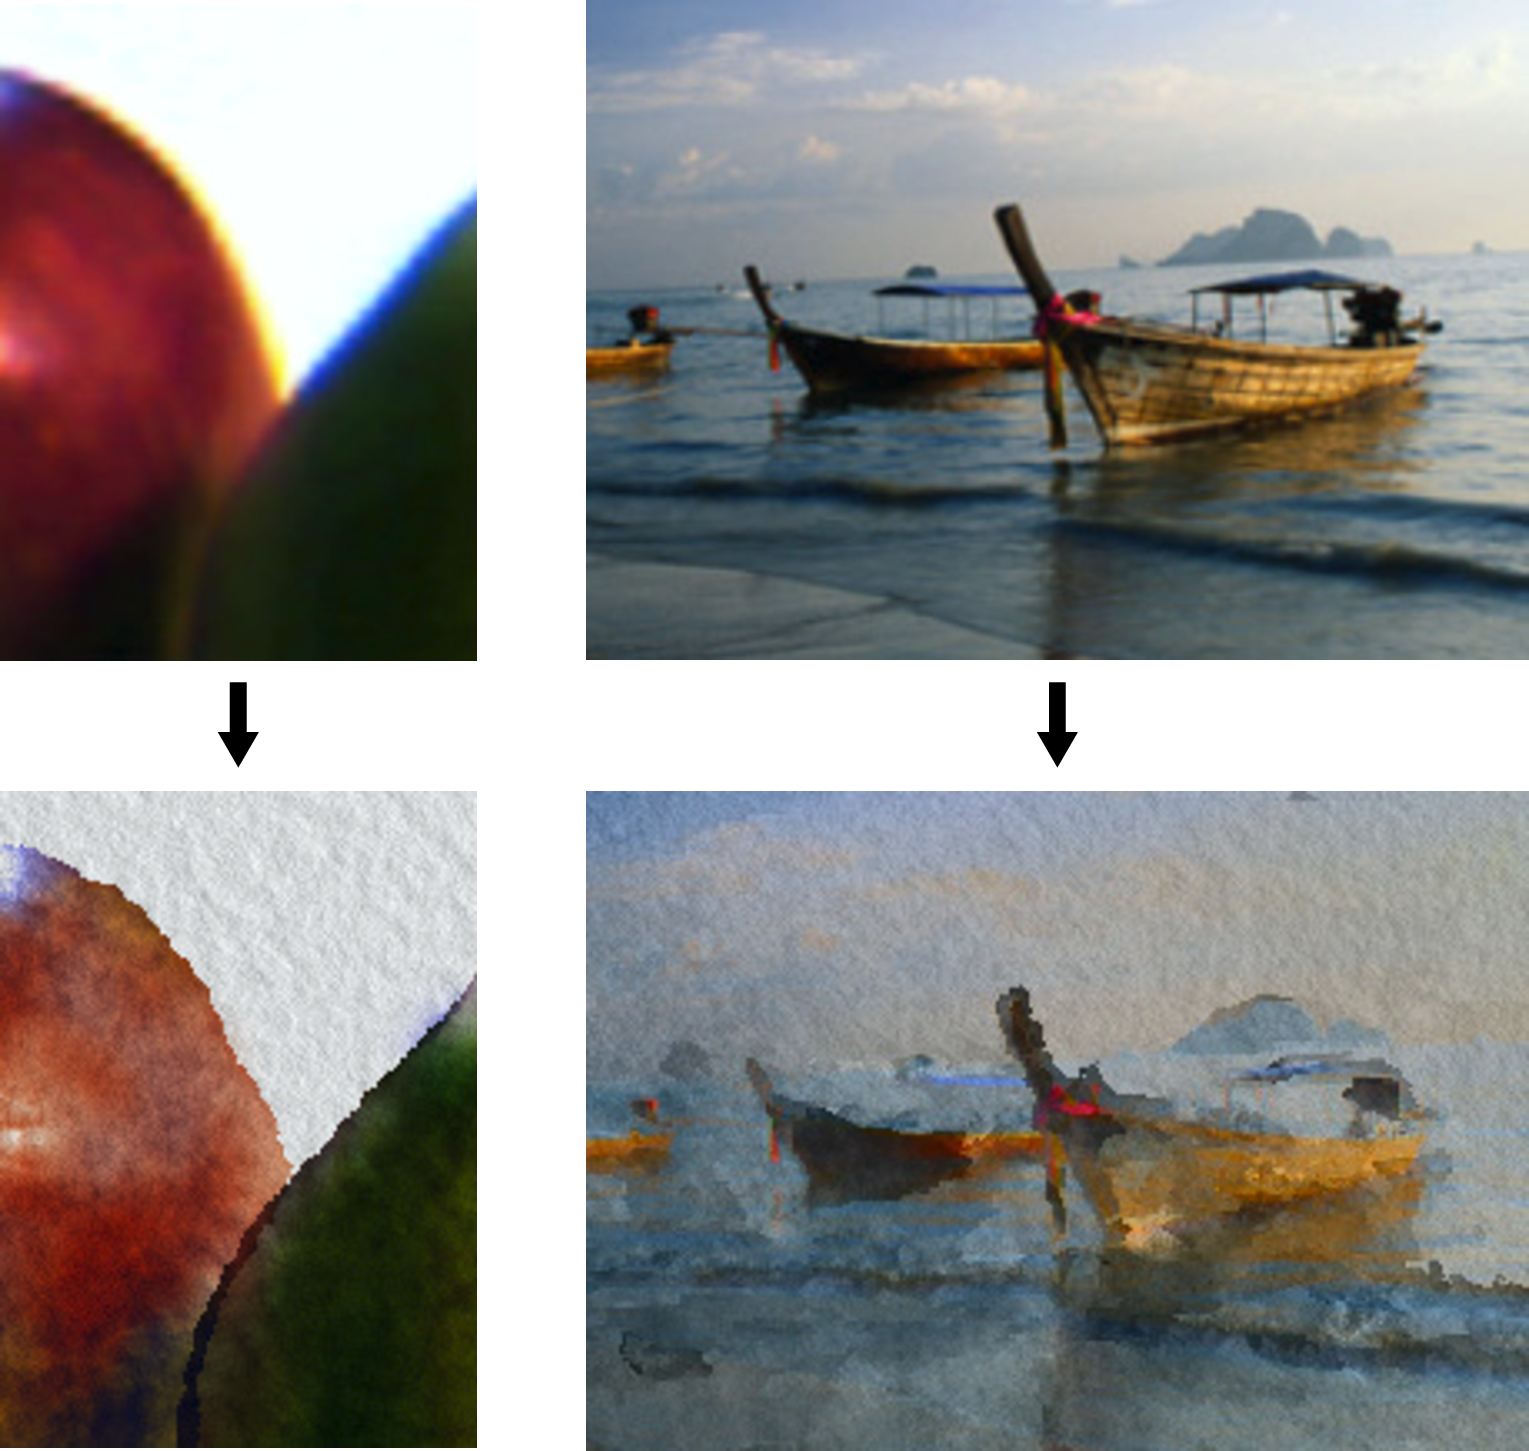
\includegraphics[width=0.45\textwidth]{figures/analogies}
	\caption{Example of image analogy: on the left is the example pair, the top right image is the input, the bottom right one is the analogy output, that transfers the style from the left pair to the image input.}
	\label{fig:analogies}
\end{figure}

\begin{figure}[ht]
	\centering
	\includegraphics[width=0.48\textwidth]{figures/colorization}
	\caption{Data recovery with image analogy: given a gray-to-color mapping (on the left), a new grayscale input is colorized (on the right). Copying directly the patches produces a blurry result (middle) whereas copying the difference of the left mapping on top of the grayscale patch produces a sharp result (bottom right).}
	\label{fig:colorize}
\end{figure}

\paragraph{Image Querying}
The increasing amount of available images has brought new algorithms for querying and processing it such as GIST and bag-of-features~\cite{Oliva01, Torralba08, Douze09}, leading to better scene detection and completion \cite{Hays07}.
Likewise, synthesis algorithms have led to new patch querying data structures (locality sensitive hashing~\cite{Gionis99}, coherency sensitive hashing~\cite{Korman11} and propagation-assisted kd-trees~\cite{He12}) and algorithms such as Patch Match~\cite{Barnes09}.
We build upon the ideas of a distributed multi-exemplar variant called PatchWeb~\cite{Barnes11}.

\paragraph{Synthesizing Stereo}
While stereoscopic data is not yet abundant~\cite{Corrigan10, Smolic10}, 
new large free rendered movies have appeared such as Elephants Dream\footnote{\url{https://orange.blender.org/}}, 
Big Buck Bunny\footnote{\url{http://bbb3d.renderfarming.net/download.html}} or 
Sintel\footnote{\url{https://durian.blender.org/}}, and efforts have been made to produce true stereo data from these for research purposes.
There have been attempts at synthesizing stereo data from monocular streams but they rely on temporal coherence to either deduce motion~\cite{Moustakas05}, use parallax cues~\cite{Zhang07} or eventually require user assistance \cite{Wang11} without leveraging external data sources.
They follow the traditional multi-view image rendering approach that consists in partially modeling the scene \cite{Seitz06, Kopf14}.

In this work, we explore the idea of image analogies applied to stereoscopic image rendering to leverage future stereoscopic image databases.